

\documentclass[11pt,a4paper,titlepage,oneside]{article}

\usepackage[most]{tcolorbox}
\usepackage{geometry}
\usepackage{hyperref} %links
\usepackage[document]{ragged2e} %floating text
\usepackage{helvet} %font
\usepackage{tocloft} % dots in table of contents sections


\usepackage{lipsum}
\usepackage{fancyhdr}


% hypthenationrules
\usepackage[T1]{fontenc}



\hypersetup{
    colorlinks,
    citecolor=black,
    filecolor=black,
    linkcolor=black,
    urlcolor=black
}
\urlstyle{same}



\geometry{
    a4paper,
    left=3cm,
    right=2.5cm,
    top=3cm,
    bottom=2.5cm
}

%remove random margin on side ? idk what happend
%\setlength{\oddsidemargin}{0pt}



%custom reusable colorbox rules
\newtcolorbox{simplebox}{colback=white, sharp corners, boxrule=1pt }


\renewcommand{\contentsname}{Sisällys} % override Contents => Sisallys on table of contents

\renewcommand{\familydefault}{\sfdefault} % set font



\renewcommand{\cftsecleader}{\cftdotfill{\cftdotsep}} % dots for sections


\def\filename{src/oppari.tex}




\newcommand\wordcount{
    \immediate\write18{texcount -sub=section \filename{} -inc  | grep Section | sed -e 's/+.*//' | sed -n \thesection p > 'count.txt'}
(\input{count.txt}words)}


\newcommand{\inputf}[1]{\def\filename{#1}\input{#1}}


\newcommand\filewcount{
    \immediate\write18{texcount -1 -sum \filename{} > count.txt }
    \input{count.txt} words }


% jos on testi definetty niin tee 
\newcommand{\istest}[2]{\ifx\testmode\undefined #2 \else #1 \fi}


% testi section näyttää word countin siltä sectionilta jos ei testi niin sitten näytä vain normaali section
\newcommand{\tsection}[2]{\istest{#1{#2\\} \wordcount \\ \medskip }{#1*{#2}}}


\newcommand{\pagesection}[1]{\istest{\section{#1}  }{\section*{#1}}}
\newcommand{\pagesubsection}[1]{\istest{\subsection{#1}  }{\subsection*{#1}}}


% adds page with everything
\newcommand{\addPage}[2]{
    \def\filename{#1}
    \pagesection{#2}
    \istest{ \filewcount \medskip }{}
    \input{#1}
}



% OPPARI SPESIFIC

\newcommand{\addPageOp}[2]{
    \def\filename{#1}
    \pagesubsection{#2}
    \istest{ \filewcount \medskip }{}
    \input{#1}
}

%lab citation style
\newcommand{\labcite}[1]{\setcitestyle{aysep={},open={(},close={.)}}\citep{#1}{}}

%lab citation style
\newcommand{\labciteend}[1]{\setcitestyle{aysep={},open={(},close={).}}\citep{#1}{}}

\newcommand{\labimgcite}[1]{\setcitestyle{aysep={},open={(},close={)}}\citep{#1}{}}

\newcommand{\hurl}[1]{\href{#1}{{\underline{\textcolor{blue}{#1}}}}}


% counter kuville
\newcounter{imgCounter}
\setcounter{imgCounter}{0}

\newcommand{\getImgCount}{
\addtocounter{imgCounter}{1}
\theimgCounter
}


% counter kaavioille
\newcounter{chartCounter}
\setcounter{chartCounter}{0}

\newcommand{\getChartCount}{
\addtocounter{chartCounter}{1}
\thechartCounter
}



\usepackage[finnish]{babel}
















% ------------------------------ BEGIN DOCUMENT ------------------------------ %
\begin{document}

\pagestyle{empty}


%------------------------------ COVER PAGE ------------------------------ %


\includegraphics[width=5cm,height=1cm]{./src/labimg.jpg}

\vspace{86mm}
\huge
\textbf{Kehityksen seuranta}
\newline

\large

\vspace{5mm}
\textbf{Oppimispäiväkirja}
\normalsize

\vspace{90mm}

LAB-ammattikorkeakoulu \newline
\vspace{2mm}
Tieto-ja tietolikenadsfklj, Insinööri (AMK) \newline
\vspace{2mm}
2024 \newline
\vspace{2mm}
Kimi Malkamäki

\newpage




%------------------------------ FIRST PAGE OF ABSTRACT ------------------------------ %
\begin{tabular}{ | l | }

    %hack for the tiivistelmä line
    \multicolumn{1}{l}{
        \begin{minipage}{6cm}
            \hspace{1mm}
            
        \end{minipage}
        \begin{minipage}{4.25cm}
            \hspace{1mm}
        \end{minipage}
        \begin{minipage}[t][1.95cm][t]{3.62cm}
            \large
            \textbf{ Tiivistelmä }
        \end{minipage}
    }\\

    \hline
    \begin{minipage}[b]{6cm}
        tekijä(t)
        \newline
        kimi malkamäki 
    \end{minipage}%
    % 2x2
    \begin{minipage}{8.5cm}
        \begin{tabular}{ | l | c | }
            \begin{minipage}[t][1cm][t]{4.25cm}
                julkaisun laji
                \newline
                Opinnäytetyö, AMK
            \end{minipage} & %
            %
            \begin{minipage}{3.62cm}
                valmistusaika
                \newline
                2024
            \end{minipage} \\ \hline%
            %
            \begin{minipage}[t][1cm][t]{4.25cm}
                sivumäärä
                \newline 
                xx+xx
            \end{minipage}
            &  \\ \hline
        \end{tabular}
    \end{minipage}%
    % end of 2x2
      \\ \hline

    \begin{minipage}[t][2cm][t]{8cm}
    Työn nimi 
        \newline 
    ammatissa kasvaminen 
        \newline 
    oppimispäiväkirja  
    \end{minipage}\\ \hline

    \begin{minipage}[t][1.5cm][t]{10cm}
    tutkinto ja koulutusala.\newline  tietoviestintätekniikka insinööri amk  

    \end{minipage}\\ \hline

    \begin{minipage}[t][7cm][t]{5cm}
    tiivistelmä: \newline lorem ipsim
    \end{minipage}\\ \hline

    \begin{minipage}[t][2cm][t]{5cm}
    avain sanat
    \end{minipage}\\ \hline

\end{tabular}

\newpage



% ------------------------------ SECOND PAGE OF ABSTRACT ------------------------------ %

tiivistelmä








\newpage


% ------------------------------ TABLE OF CONTENTS ------------------------------ %

%keep page numbers off
\setcounter{page}{0}
\pagestyle{empty}
\pagenumbering{gobble}

\tableofcontents





\newpage



% ------------------------------- TERMISTÖ ------------------------------- %


TERMISTÖ

mitä termejä käytetään


ECMAscript                  skriptaus-kieli standardi 


\newpage





% ------------------------------- CONTENT PRELUDE COMMANDS ------------------------------- %
%enable page counting
\pagenumbering{arabic}
\clearpage
\setcounter{page}{1}

%set heaader and footer
\pagestyle{fancy}
%%
\lfoot{}
\cfoot{}
\rfoot{}
%%
\lhead{}
\chead{}
\rhead{\thepage}
%%
\renewcommand{\headrulewidth}{0pt}
\renewcommand{\footrulewidth}{0pt}
%\newcommand{\n}{\newline\vspace{20mm}}


\section{Johdanto}              % ------------------------------- JOHDANTO ------------------------------- %


%tuleeko tähän oikeasti preamble itse tekniikan alasta 

Opinnäytetyön tavoitteena on seurata kehittymistä 13 viikon seurantajakson aikana työharjoittelussa 
ja tutkia henkilökohtaista kehitystä harjoituksen aikana.
\medskip


opinnäite työ on päiväkirjamallinen ja liitteenä on päiväkirja dokumentti, 
johon olen kirjannut mitä olen tehnyt, mitä olen oppinut ja minkälaisten teknologioiden kanssa olen ollut tekemisissä.
\medskip


työ toteutettiin Starttaamo Oy:ssä, suomalaisessa startup yrityksessä, joka pyrkii ratkomaan ongelmia työergonomian kanssa.
Pää tavoitteena on vähentää sairaslomia saamalla työntekijät noudattamaan, alojen ammattilaisten suunnittelemien liikunta- ja ruokavalio-ohjelmia. 
% jotain selitystä itse alustasta jonka kanssa tulen tekemiseen
Yrityksen pää myyntituote on alusta, jonka kanssa tulen tekemään töitä.


\medskip






\newpage
\section{Lähtötilanne}         % ------------------------------- LÄHTÖTILANNE ------------------------------- %


ennen opinnäytetyön kirjoittamista ja seurantajakson alkamista. 

% kauan olen ollut opiskelija
Olen opiskellut LAB ammattikorkeakoulussa XX lukukautta ja olen kirjoitusen aikana neljännen vuoden tieto- ja tietoviestintätekniikkan opiskelia.
% jotain lorem siitä että olen oppinut koulusssa jotain
%
% jotain siitä että ei ole oikeaa työ kokemusta vaikka on vahva koodauspohja
Minulla ei ennen harjoitusta ollut aijempaa työkokemusta alalta. 
% selitä paremmin.. mitä kaikkea itse projektissa tullaan tekemään ja miten voin oppia asioista
projektissa käytettään monta teknologiaa jonka kanss en ole ollut tekemisessä joten niiden oppiminen tulee uutena
\medskip







\newpage
\section{Teoria}                % ------------------------------- TEORIA ------------------------------- %



\subsection{Kehitys ympäristö / Teknologia pino}

Startupit haluaa nopeaa liikkumista ja kehittymistä ja se näkyy teknologia valinnoissa.
projekti käyttää fullstack frameworkkia meteor joka on suunniteltu nopeaan kehittelyyn ja käyttöönottoon.
\medskip

käyttöliittymä on toteutettu käyttämällä reactjs kirjastoa
\medskip

projektin tietokanta on mongodb, joka tekee uusien collectioneiden tekemisestä helppoa sillä nosql kantoihin ei travitse määritellä skeemaa.
\medskip










\newpage
\subsection{Meteor}                % ------------------------------- Meteor ------------------------------- %



\subsubsection{Mikä on meteor}


%https://github.com/mongodb/mongo?tab=License-1-ov-file
% mongo licence 

% https://github.com/meteor/meteor?tab=License-1-ov-file
% meteor lisence

% https://guide.meteor.com/collections.html#mongo-collections
% meteor uses mongo. but it is not manditory



%tässä blokissa on tarpeeks tekstiä kuhan sen kirjottaa kunnoll


%src meteor homepagef
Meteor on full-stack JavaScript web-framework ja on itsessään avoimeen lähdekkoodiin perustuva, 
poislukien meteorin mukaan paketoimaa mongodb tietokantaa, joka toimii Server Side Public Lisenssillä.
Meteor on suunniteltu nopeaan kehittämiseen monelle laitteille ja nopeaan käyttöönottoon.
%
% https://www.meteor.com/
% viitattu 28.5 ...
% pakota ... frontend teknologiaa ... kehittäjää? mahdollisesti ei tätä edes kun mmeillä on alempana toi featuret
%Meteor ei pakota kehittäjää käyttämään tiettyä front-end teknologiaa vaan sillä on integraatio moneen yleiseen frontend-framework:kiin, kuten Vue, React, Svelte tai Angular.
\medskip


    
% https://www.meteor.com/
% viitattu 28.5

Meteor tukee monta ominaisuutta kuten.
\begin{itemize}
    \item tukee monta Front-end kirjastoa ja frameworkkkia
    \item tukee typescriptiä
    \item sisään rakennettu käyttäjä systeemi
    \item toimii monella laitteellqa
    \item helppo ja nopea käyttöönottaa 
\end{itemize}




\subsubsection{Meteor metodit}

% kirjoita tämä oikeella oppari tyylillä. idk tuntuu vähän väärältä tässä



% kappale rpc. mikä on ja miten eroaa restful

%enemmän yleis selostusta rps ja restful mikä on ero hyvät ja huonot puolet

Meteor ei käytä RESTful rajapintaa vain RPC (eng Remote procedure call) rajapintaa. 
%uusiks
Tarkoittaa että client kutsuu funktioita palvelimella meteorin kautta.
%uusiks jotenkin huono 
Palvelimelle määritetään metodit, joita voidaan kutsua palvelimelta tai clientiltä.




\medskip


% ehk uusiks
Methodit suoritetaan ja määritetään funktioina palvelimen puolella, ja niitä voi kutsua clientistä tai palvelimelta.
% uusiks ainakin alku. 
Metodit antavat kutsujasta tietoa, esim. onko kutsuja kirjautunut sisään ja jos on niin mikä on hänen käyttäjätunnuksensa. 
%uusiks
Näin voi helposti katsoa onko kutsujalla tai käyttäjällä oikeuksia metodin kutsumiseen.








\newpage
\subsection{React}                % ------------------------------- REACT ------------------------------- %
\wordcount


%ei varmaan saa olla kysymy
\subsubsection{Mikä on React}

%ei saa olla metatekstiä
%https://github.com/facebook/react/blob/main/README.md
%https://www.infoq.com/news/2013/06/facebook-react/
% molemmat siteerattu 27.5.24


% ei ole metan kehittämä vaan se on vaan ylläpitämä. facebookin työntekijä teki sen
React on metan kehittämä ja ylläpitämä avoimeen lähdekoodiin perustuva javascript kirjasto, joka on suunniteltu reaktiivisien käyttöliittyjien kehittämiseen.
%more text

%rnative selitys paremmin
reaktia voi käyttää web ja mobiili käyttöliittymien tekemiseen react nativella
%vitusti lisää tekstiä
\medskip








\subsubsection{jsx}

%https://react.dev/learn/writing-markup-with-jsx
%https://facebook.github.io/jsx/ 

% jsx = js xml
% https://medium.com/@sjarancio/what-is-jsx-e3dda0af3490

%transpilation
%https://www.scholarhat.com/tutorial/react/getting-started-with-jsx
% https://www.typescriptlang.org/docs/handbook/jsx.html

% kaikki viitattu 27.5

%html koodia uusiks
JSX (javascript XML) on sytaksi jatke javascriptille, joka antaa kehittäjän kirjoittaa html tyylistä koodia javascriptin sekaan
% asiakielellä
selain ei itse osaa lukea jsx koodia joten se pitää transpiloida javascriptiksi ennen kun sen voi deploy



% suora sitaatti https://facebook.github.io/jsx/ 
JSX ei ole ECMAscript standardissa, joten selaimet eivät osaa tulkita sitä, vaan JSX se on suunniteltu transpiloitavaksi johonkin ECMAscript standardia toteuttavalle kielelle
\medskip

\bigskip
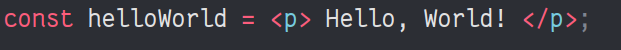
\includegraphics[width=10cm]{src/public/oppar/pure_jsx_example.png}

Kuva 1. kuvankaappaus JSX syntaxista.
\medskip

Kuvassa luodaan elementti helloWorld, jolle annetaan arvoksi paragraafi, jossa teksti "Hello, World!"{}.
% loppu pitää kirjottaa jotenkin paremmin ja pitää yhistää paremmin 
Elementtien arvot voidaan kirjoittaa html tyylillä, joka tekee jutuista kivaa.
\medskip



\bigskip

\includegraphics[width=15cm]{src/public/oppar/transpiled_jsx_example.png}

Kuva 2. Kuvankaappaus helloWorld elementistä, joka on käännetty javascriptiin. 
\medskip

%vähän toistoa muttei väliä sillä pitää siteerata tämä

%https://babeljs.io/repl 
kuvassa on helloworld elementti, joka on käännetty natiiviksi javascriptiksi babel kääntäjää käyttäen.
Tämä antaa selaimille mahdollisuuden tulkita JSX koodia.
%jotain lisää
\medskip

% https://github.com/facebook/react/blob/a4195750779dbd9a13e1615fbbd493bf2c5768ca/packages/react/src/ReactElement.js#L362
%pitää vissii kysyy voiko lähdekoodia käyttää lähteenä..


\subsubsection{Komponentit}


%https://react.dev/learn/your-first-component

Oma tekemä komponentti. se voi sisältää tilaa ja kutsuja muihin komponentteihin jne
komponentteihin voi lisätä interaktiivisuutta jne



komponentit on vähän niinkuin oma elementti jonkqa voi kirjoittaa jsx koodiin siististi

\medskip

\subsubsection{Reaktin struktuuri}
index.js lähtien
reactdom createroot
root.render
käy läpi kaikki lapset mitkä kaikilla componenteilla on ja tekee niistä natiivi html elementtejä jotka sitten selain renderöi. 

koko react läpi jsx kooditsta htmllään
\medskip



\subsubsection{VDOM}


%jotain domista, mikä se on ja miten se liittyy käyttöliittymiin ja sitten mikä on vdom
% vai pitäisikö samantien aloittaa että meillä on vdom, ja sittem selittää mikä dom on..... kuulostaa väärältä

virtuaali dom (document object model) on virtuaali representaatio oikeasta domista, 
dom on puu mainen struktuuri koko dokumentista


%https://medium.com/@BharathkumarV/reacts-virtual-dom-17fdcb290a10
% siteerattu 27.5

%selittää vähän paremmin ja tuntuu että puu struktuurinen ei ole oikein hyvä tapa kuvata domia
DOM (eng Document object model) on puu-struktuurinen representaatio koko käyttöliittymästä.
Tätä struktuuria käytetään rajapintana javascriptin ja html:län välillä. jotain jotain hidas.
%
VDOM (eng Virtual Dom) on virtuaalinen esitys domista jonka react pitää musitissaan koko suorituksen ajan.
vdomia käyttäen react voi nopeasti päätellä mitkä osat käyttöliittymästä pitää päivittää.
kun jonkun komponentin tila päivittyy react voi päivittää 






\newpage
\subsection{Mongodb}

%src mongo lisence.


% https://www.techtarget.com/searchdatamanagement/definition/MongoDB
% jotain täältä. tämä tosin sanoo että on open source joka ei oo sinänsä totta
% sitaatti 28.5


mongodb on Server Side Public Lisenssillä toimiva NoSql dokumentti pohjainen tietokanta.% datambase management program? 
%en tiedä onko edes järkee mainita
mongo tukee ajureita monelle suositulle kielelle

mongodb collection

"horisonttaali" skaalautuminen

helppo third party support
aka helposti integroitava





\subsection{Responsiiviset käyttöliittymät}
responsiivinen käyttöliittymän kehitys lorem ipsum






\subsection{Lokalisaatio}
lorem

\subsubsection{i18n}
en tiedä saanko hirveesti kirjotatteu
jos en niin kaada tämä ylempään
tai jos ei tule toista subsub sectionia










\newpage
\section{Toteutus}              % ------------------------------- TOTEUTUS ------------------------------- %


\subsection{Lokalisaatio}
käännös ja lokalisaatio


\subsection{Uuden ominaisuuden lisäys}
ipsum progressio multiseuranta feature lisäys



\section{Yhteenveto}

sehän meni ihan hyvin 

opin käyttämään projektissa käytettyjä teknologioita

opin tekemään töitä ammatillisessa työympäristössä




\newpage
\section{Lähteet}               % ------------------------------- LÄHTEET ------------------------------- %

miten laitan liitteen päiväkirjasta ja millainen se pitäisi olla





\end{document}



